\documentclass{beamer}
\usefonttheme[onlymath]{serif}

\usepackage{amsfonts}

% Code Block Setting
\usepackage{listings}
\lstset{language=C,
numberstyle=\footnotesize,
basicstyle=\ttfamily\footnotesize,
numbers=left,
stepnumber=1,
frame=shadowbox,
breaklines=true}

\usetheme{Warsaw}
% \usecolortheme{dove}

% Add frame number and total frame number in footline
\defbeamertemplate*{footline}{shadow theme}{%
    \leavevmode%
    \hbox{\begin{beamercolorbox}[wd=.5\paperwidth,ht=2.5ex,dp=1.125ex,leftskip=.3cm plus1fil,rightskip=.3cm]{author in head/foot}%
            \usebeamerfont{author in head/foot}\hfill\insertshortauthor
        \end{beamercolorbox}%
        \begin{beamercolorbox}[wd=.4\paperwidth,ht=2.5ex,dp=1.125ex,leftskip=.3cm,rightskip=.3cm plus1fil]{title in head/foot}%
            \usebeamerfont{title in head/foot}\insertshorttitle\hfill%
        \end{beamercolorbox}%
        \begin{beamercolorbox}[wd=.1\paperwidth,ht=2.5ex,dp=1.125ex,leftskip=.3cm,rightskip=.3cm plus1fil]{title in head/foot}%
            \hfill\insertframenumber\,/\,\inserttotalframenumber
    \end{beamercolorbox}}%
    \vskip0pt%
}

% Tikz related
\usepackage{tikz}
\usetikzlibrary{fit}
\usetikzlibrary{calc}
\usetikzlibrary{positioning}

% Number the figures
\setbeamertemplate{caption}[numbered]

% Add outline page at begining of each section
\AtBeginSection[]
{
    \begin{frame}<beamer>
        \frametitle{Outline}
        \tableofcontents[currentsection, hideallsubsections]
    \end{frame}
}

%%%%%%%%%%%%%%%%%%%%%%%%%%%%%%%%%%%%%%%%%%%%%

\title{Parallel Approaches to the String Matching Problem on the GPU}
\author{
    Saman Ashkiani\inst{1},\\
    Nina Amenta\inst{1},\\
    John D. Owens\inst{1}
}
\institute{
    \inst{1} University of California, Davis
}
\date{
    \tiny{28th ACM Symposium on Parallelism in Algorithms and Architectures}\\
    \tiny{Presented by Shiang-Yun Yang}
}

\begin{document}
\begin{frame}
    \titlepage
\end{frame}

\section{Introduction}

\subsection{Sparse Matrix Vector Multiplication}
\begin{frame}
    \frametitle{Definition and Propety}
	\begin{itemize}
		\item A sparse matrix is a matrix in which most of the elements 
			are zero.
		\item Sparse data is by nature more easily compressed and thus 
			require significantly less storage.
			\begin{itemize}
				\item Many formats have been proposed, such as CSR, 
					CRS, DIL, and so on.
			\end{itemize}
	\end{itemize}
\end{frame}

\subsection{CSR Format}
\begin{frame}[fragile]
	\frametitle{Compressed Row Storage}
	\begin{align*}
		A = \begin{bmatrix}
			0 & 0 & a & 0 & 0 & 0 & b & c \\
			0 & 0 & d & e & 0 & 0 & f & 0 \\
			0 & 0 & 0 & 0 & g & h & i & j \\
			k & l & 0 & 0 & m & n & o & p \\
		\end{bmatrix}
	\end{align*}
	\begin{table}[]
		\centering
		\caption{CSR format}
		\label{my-label}
		\begin{tabular}{l | c | c | c | c | c | c | c}
			\hline
		index & 0 & 1 & 2 & $\cdots$ & 12 & 13 & 14 \\ \hline
		val      & a & b & c & $\cdots$ & m & n & p  \\ \hline
		col\_ind & 2 & 6 & 7 & $\cdots$ & 4 & 5 & 7 \\ \hline
		\end{tabular}
		\\
		\begin{tabular}{l | c | c | c | c | c}
			\hline
		rowptr      & 0 & 3 & 6 & 10 & 15 \\ \hline
		\end{tabular}
	\end{table}
\end{frame}

\subsection{Serial Implementation Example}
\begin{frame}[fragile]
	\frametitle{Serial Implementation Example}
	\begin{itemize}
		\item $A_{n,m} \times x_{m,1} = y_{n,1}$
\begin{lstlisting}
for (i = 0; i < n; ++i) {
    double y0 = y[i];
    for (k = rowptr[i]; k < rowptr[i+1]; ++k)
        y0 += val[k] * x[column_index[k]];
    y[i] = y0;
}
\end{lstlisting}
	\end{itemize}
\end{frame}

\subsection{Changes of Parallel Implementation}
\begin{frame}
	\frametitle{Changes of Parallel Implementation}
	\begin{itemize}
		\item Bandwith
			\begin{itemize}
				\item the upper bound of $\text{FLOPS}\footnote{Floating-Point Operations Per Second }:\text{BYTES} = 0.25$
			\end{itemize}
		\item Load imbalance
			\begin{itemize}
				\item The non-zeros in a matrix may not be evenly distributed 
					across different rows.
				\item The matrix data have low reuse. Each non-zero element 
					is only once for computing the corresponeding dot product.
			\end{itemize}
	\end{itemize}
\end{frame}

\subsection{Executive Summary}
\begin{frame}
	\frametitle{Executive Summary}
	\begin{itemize}
		\item Improve the bandwidth by block-based compressed common
			coordinate format.
		\item Addressing the load imbalance problem by customized
			efficient segmented scan/sum.
		\item Using auto-tuning framework to explore optimization parameter 
			for different sparse matrices and different platforms.
	\end{itemize}
\end{frame}


\section{Preliminaries}

\subsection{Basic Scenario}
\begin{frame}
	\frametitle{Basic Scenario}
	\begin{itemize}
		\setlength\itemsep{1em}
		\item Binary pattern of length $m$: 
			$X = x_0 \; \cdots \; x_{m-1}$
		\item Binary text of length $n$ ($n \ge m$): 
			$Y = y_0 \; \cdots \; y_{n-1}$
		\item Substring of $Y$: $Y[r] = y_r y_{r+1} \cdots y_{r+m-1}$
		\item Our Objective is to find all indices $r$ such that 
			$Y[r] = X$ for $0 \le r < n-m+1$.
	\end{itemize}
\end{frame}

\subsection{Graphic Processing Units}
\begin{frame}
	\frametitle{Graphic Processing Units}
	\begin{itemize}
		\item Both a computational hierarchy and a memory hierarchy.
		\item CUDA programming model
	\end{itemize}
\end{frame}

\subsection{Serial Rabin-Karp}
\begin{frame}
	\frametitle{Definition}
	For any $X \in \{0, 1\}^m$ :
	\begin{itemize}
		\setlength\itemsep{1em}
		\item $F(X) = 2^{m-1} x_0 + \cdots + 2 x_{m-2} + x_{m-1}$
		\item Pick a random prime number $p \in (1, mn^2)$
				$$F_{p}(X) \overset{p}{\equiv} F(X)$$
		\item Define two matrices,
			\begin{align}
				K(0) = \begin{bmatrix}
					1 & 0 \\ 
					1 & 1
					\end{bmatrix}, \;
				K(1) = \begin{bmatrix}
				1 & 1 \\ 
				0 & 1
				\end{bmatrix}
			\end{align}
		\item The fingerprint of $X$ is 
			$K(X) = K(x_0) \cdots K(x_{m-1})$.
	\end{itemize}
\end{frame}

\begin{frame}
	\frametitle{The RK Algorithm}
	\begin{description}
		\setlength\itemsep{1em}
		\item[(1)] Choose a random prime number $p \in (1, mn^2)$.
		\item[(2)] Compute fingerprints $F_p(X)$ and $F_p(Y[r])$ for 
			$r \in [0, n-m+1)$
		\item[(3)] Compare: if $F_p(Y[r])$ and $F_p(X)$ are equal,
			then $X$ and $Y[r]$ are equal with high probability, 
			otherwise there is no match.
	\end{description}
\end{frame}

\begin{frame}
	\frametitle{Compute Efficiently in Step 2}
	\begin{itemize}
		\item $F_p(Y[r+1])$ can be computed by using $F_p(Y[r])$:
			\begin{align}
			F_p(Y[r+1]) \overset{p}{\equiv} 2 (F_p(Y[r]) - 2^{m-1} y_r) + y_{r+m+1}
			\end{align}
		\item Compute $K_p(Y[r+1])$ based on $K_p(Y[r])$:
			\begin{align}
			K_p(Y[r+1]) \overset{p}{\equiv} A_p(y_r) K_p(Y[r]) K_p(y_{r+m+1})
			\end{align},
			where $A_p(x)$ is defined as the left inverse of $K_p(x)$ for any binary value $x \in \{0, 1\}$.
	\end{itemize}
\end{frame}



\section{Strategy}

\subsection{Cooperative Rabin-Karp}
\begin{frame}
	\frametitle{Definition}
	\begin{itemize}
		\item We define $\mathcal{S}$ and $\mathcal{T}$ vectors 
		as follow:
	\end{itemize}
	\begin{figure}
		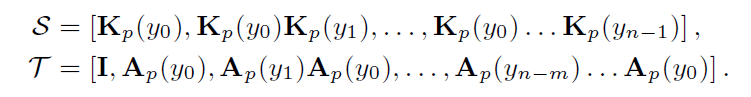
\includegraphics[scale=0.50]{figure/fig-ST.png}
	\end{figure}
	\begin{itemize}
		\item With $p$ processors, a scan can be computed in 
			$O(n/p + \log p)$ time steps.
	\end{itemize}
\end{frame}


\begin{frame}
	\frametitle{Final Result}
	\begin{figure}
		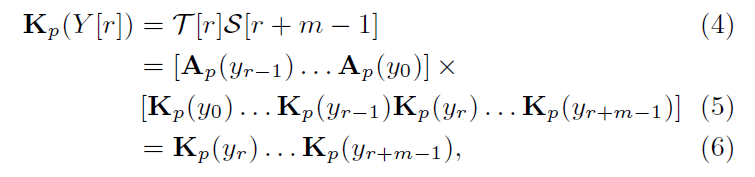
\includegraphics[scale=0.50]{figure/fig-Kp.png}
	\end{figure}
	\begin{itemize}
		\item Scan operation can be computed cooperatively by a set of 
		independent threads or processors.
	\end{itemize}
\end{frame}

\subsection{Divide-and-Conquer Rabin-Karp}
\begin{frame}
	\frametitle{Divide and Conquer}
	\begin{itemize}
		\setlength\itemsep{1em}
		\item These parallel scans require intermediate communication
		 between different processors and cores.
		\item Assign different parts of the text of different 
		processors and process each part seperately. The final result
		is simply a union of matching results for each subproblem.
	\end{itemize}
\end{frame}

\begin{frame}
	Let $L$ denote the number of subtexts. Then, if we
	show each subtext as $Y^l$, for $0 \le l < L$, the division
	process can be shown as:
	\begin{figure}
		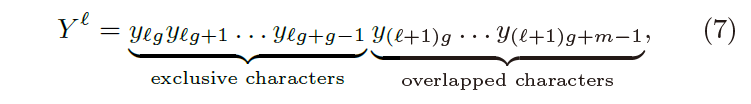
\includegraphics[scale=0.50]{figure/fig-DC.png}
	\end{figure}
	where each subtext has $g = (n-m+1)/L$ \textit{exclusive} 
	characters, plus $m-1$ \textit{overlapped} characters.
	\begin{itemize}
		\item If $L = 1$, DRK will be identical to CRK.
	\end{itemize}
\end{frame}

\subsection{Hybrid Rabin-Karp}
\begin{frame}
	\begin{itemize}
		\setlength\itemsep{1em}
		\item We define \textit{Hybrid RK} (HRK) as a method in which 
		the main text is divied into subtexts (Eq. (7)) and then each 
		subtext is assigned to a group of processors.
		\item If $L = 1$, HRK will be identical to CRK.
	\end{itemize}
\end{frame}

\begin{frame}
	\begin{figure}
		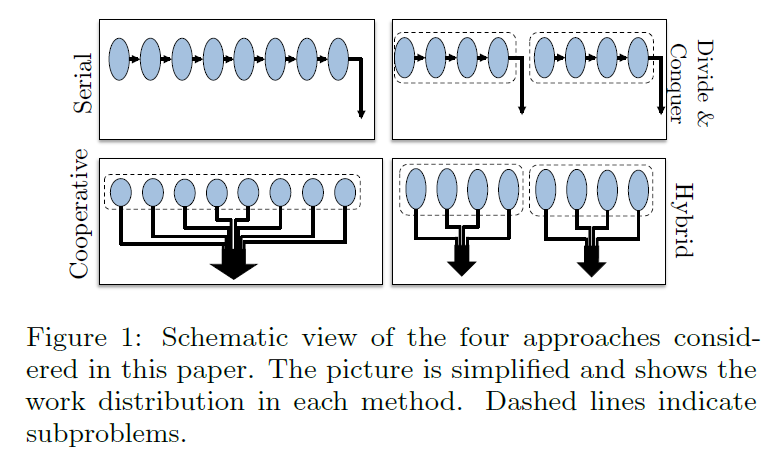
\includegraphics[scale=0.50]{figure/fig-all.png}
	\end{figure}
\end{frame}

\subsection{Theoretical Analysis}
\begin{frame}
	\begin{itemize}
		\setlength\itemsep{1em}
		\item The finite number of $p$ processors.
		\item Assume that all processors have access to a globally 
		shared memory.
	\end{itemize}
	\begin{figure}
		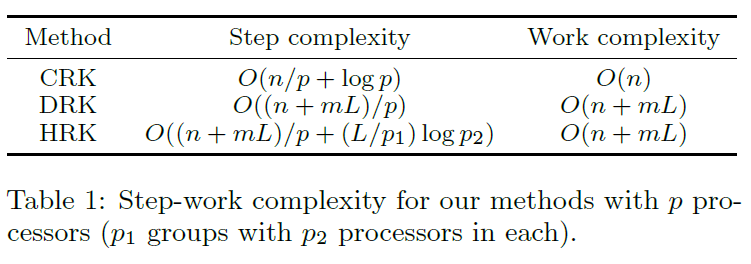
\includegraphics[scale=0.40]{figure/fig-complexity.png}
	\end{figure}
\end{frame}

\end{document}
